\documentclass[11pt,a4j,fleqn]{jarticle}
\usepackage{amsmath,amsthm,amssymb}
\usepackage[dvipdfmx]{graphicx}

\title{包絡線定理}
\author{YOON SEUNGWON}
\date{2013.06.06}


\begin{document}

\maketitle

\section{包絡線定理}

tをパラメターとする微分可能な関数$f(x,t)$が与えられたとき,
\begin{equation}
f(x,t) = 0\label{eq:square-1}
\end{equation}
によって曲線群が定まる.すなわち,$t$をある値に固定すれば,(1) を満たす$x$の関係を
表す曲線(今の場合は直線)が 1 つ定まる.$t$ も値を変えれば,別の曲線が定められるので,(1) は $t$をパラメター
とする曲線群を示していると考えられる.$t$を連続的に変えたとき,この曲線の位置や形は連続的
に変れる.ある曲線が,上の各曲線 (1)に接し,しかも接点の軌跡となっているとき,その曲線
(1)を満たす曲線群の包絡線という.




\section{Pythonプログラムコード}
ここでは、基本の例として$f(x,t)=tx-t^2$の包絡線を導くために作ったコードについて説明する。
$t$の範囲を与えて、その最小値から最大値までの直線を跡を残しながら順番に引いて行くアニメーション効果を表すコードになっている。

\begin{quote}
\begin{verbatim}
# Animation using generator in FuncAnimation
import matplotlib.pyplot as plt
from matplotlib import animation
import numpy as np

# Define constants
VERSION = 1
if VERSION == 2:
    # plt.axes(xlim=(-x_Bound, x_Bound), ylim=(y_Lower, y_Upper))
    x_Bound = 35
    y_Lower, y_Upper = -100, 200
    # x = np.array([x_Min, x_Max])
    x_Max = 50
    x_Min = -x_Max
    # t = -t_max, -t_max + 1, ..., t_max
    t_Max = 20
    Interval_ms = 80
elif VERSION == 3:
    x_Bound = 50
    y_Lower, y_Upper = -100, 600   
    x_Max = 50
    x_Min = -x_Max 
    t_Max = 60
    Interval_ms = 50
else:
    VERSION = 1   
    x_Bound = 20
    y_Lower, y_Upper = -50, 100
    x_Max = 50
    x_Min = -x_Max
    t_Max = 8
    Interval_ms = 100

fig = plt.figure()
ax = plt.axes(xlim=(-x_Bound, x_Bound), ylim=(y_Lower, y_Upper))
ax.axhline(linewidth=2.0, color="black")
ax.axvline(linewidth=2.0, color="black")
fig.suptitle('Envelope Theorem.ver' + str(VERSION), fontsize=20)
plt.xlabel('x', fontsize=16)
plt.ylabel('y', fontsize=16)
ax.grid()
line, = ax.plot([], [], 'r-', lw=4)

def f():
    line.set_data([], [])
    return line,

def t_gen():
    t = -t_Max
    while t <= t_Max:
        yield t
        t += 1

def animate(t):
    x = np.array([x_Min, x_Max])  # Two points are enough to determine a line
    y = t*x - t**2
    ax.plot(x, y, 'b-')
    line.set_data(x, y)
    return line

anim = animation.FuncAnimation(fig, animate, t_gen, init_func=f,
                               interval=Interval_ms, blit=False, repeat=False)

plt.show()
\end{verbatim}
\end{quote}

\section{自分のpythonコードの改善点}
アニメーション効果は、pythonのガイドやWEBページでの説明を参考にするとその形式を作るのは簡単である。
重要なことは関数の形をどう定義するかだと思う。
その改善点としては、上述したコードだと三つの場合しか表せない。
故に、$t$の範囲の設定がバージョンごとに三つしか出来ないので一般的な形だとは言えない。
本当は、$t$の値から$x$の範囲や$y$の範囲も求めさせる計算式を作るべきである。


\begin{figure}[b]
 \begin{minipage}{0.5\hsize}
  \begin{center}
   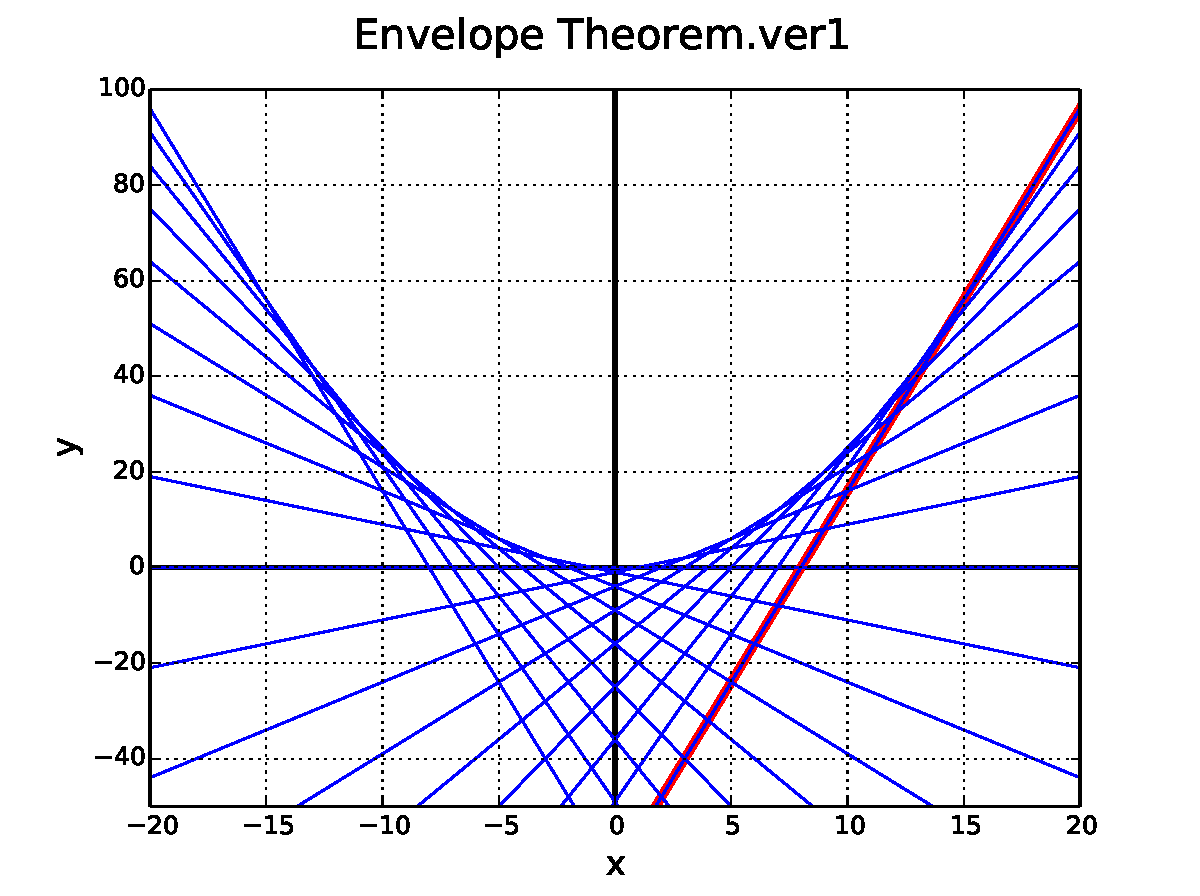
\includegraphics[width=13mm]{envelope0.pdf}
  \end{center}
  \caption{一つめの図}
  \label{fig:one}
 \end{minipage}
 \begin{minipage}{0.4\hsize}
  \begin{center}
   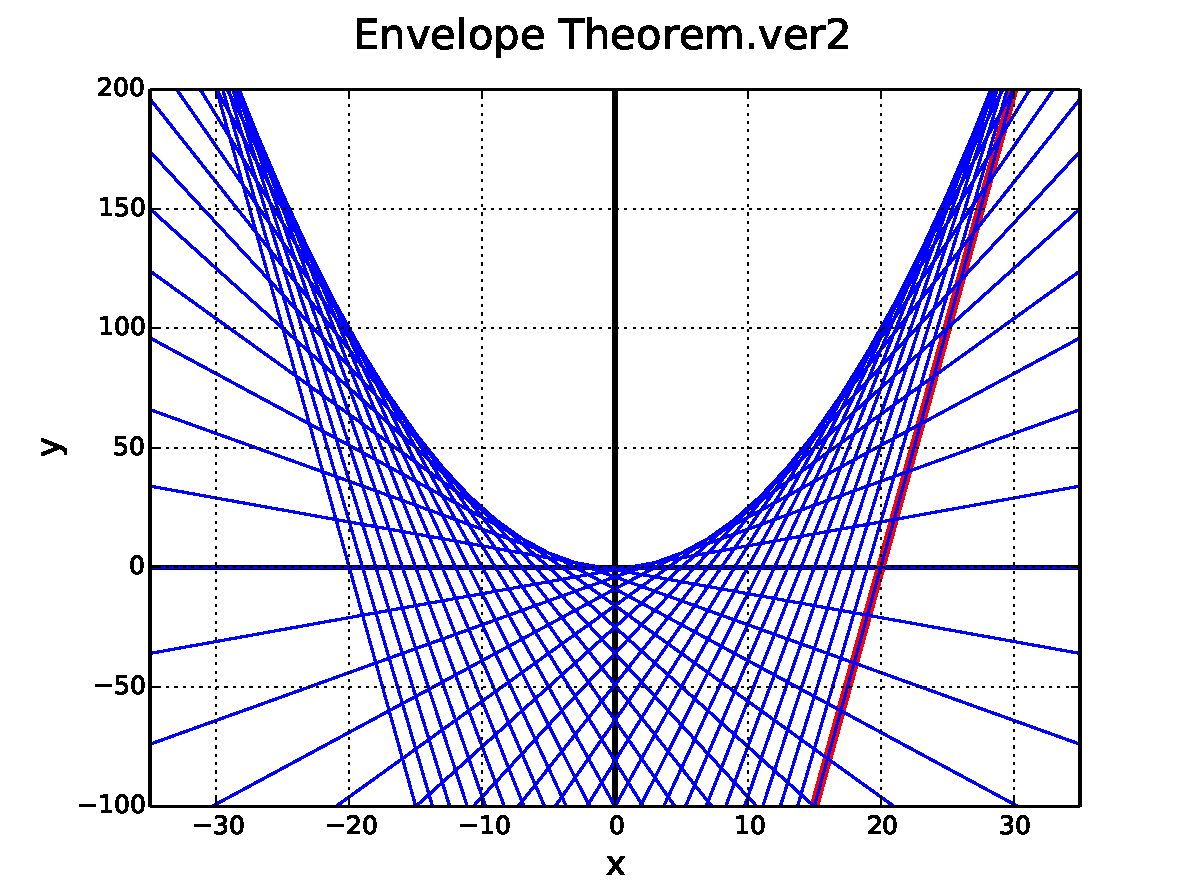
\includegraphics[width=13mm]{envelope1.pdf}
  \end{center}
  \caption{二つめの図}
  \label{fig:two}
 \end{minipage}
\end{figure}


\begin{thebibliography}{0}
\bibitem{OyamaYasuda11}
尾山大輔・安田洋祐「経済学で出る包絡線定理」『経済セミナー』2011年10・11月号.

\end{thebibliography}

\end{document}